\documentclass[autodetect-engine,dvipdfmx-if-dvi,ja=standard,everyparhook=compat]{bxjsarticle}

\usepackage{graphicx}        % 図を表示するのに必要
\usepackage{color}           % jpgなどを表示するのに必要
\usepackage{amsmath,amssymb} % 数学記号を出すのに必要
\usepackage{type1cm}         % fontsizeのエラー回避
\usepackage{here}            % 図の強制配置
\usepackage{url}             % URLをいい感じにしてくれる
\usepackage{subfigure}       % 図をまとめて表示
\usepackage{pdfpages}        % PDFの連結
\usepackage{setspace}
\usepackage{cases}
\usepackage{fancyhdr}
\usepackage{wrapfig}% 図の回り込み


% 余白の設定
% \setlength{\textheight}{\paperheight}   % 紙面縦幅を本文領域にする(BOTTOM=-TOP)
% \setlength{\topmargin}{-15.4truemm}     % 上の余白を10mm(=1inch-15.4mm)に
% \addtolength{\topmargin}{-\headheight}  %
% \addtolength{\topmargin}{-\headsep}     % ヘッダの分だけ本文領域を移動させる
% \addtolength{\textheight}{-20truemm}    % 下の余白も10mm
% \setlength{\textwidth}{\paperwidth}     % 紙面横幅を本文領域にする(RIGHT=-LEFT)
% \setlength{\oddsidemargin}{-5.4truemm}  % 奇数ページの左の余白を20mm(=1inch-5.4mm)に
% \setlength{\evensidemargin}{-5.4truemm} % 偶数数ページの左の余白を20mm(=1inch-5.4mm)に
% \addtolength{\textwidth}{-40truemm}     % 右の余白も20mm

% タイトル
\title{タイトル}

% ヘッダとフッタの設定
% \lhead{電気電子情報工学実験}
% \chead{}
% \rhead{20315784 佐藤凌雅}
% \lfoot{}
% \cfoot{\thepage} % ページ数
% \rfoot{}

\parindent = 0pt  % 行頭の字下げをしない
\setstretch{1.0}  % 行間

% キャプションの英語化
\renewcommand{\figurename}{Fig.}
\renewcommand{\tablename}{Table}

% 各章,節などタイトルの大きさを変更
% \titleformat*{\section}{\Huge\bfseries}
% \titleformat*{\subsection}{\Large\bfseries}

% 式の番号を(senction_num.num)のようにする
% \makeatletter
% \@addtoreset{equation}{chapter}
% \def\theequation{\thechapter.\arabic{equation}}
% \makeatother

% 呼び出したページのページ番号を消す
\newcommand{\deletePageNum}{
    \thispagestyle{empty}
    \clearpage
    \addtocounter{page}{-1}
}

% urlのフォントを直す
\renewcommand\UrlFont{\rmfamily}


\begin{document}
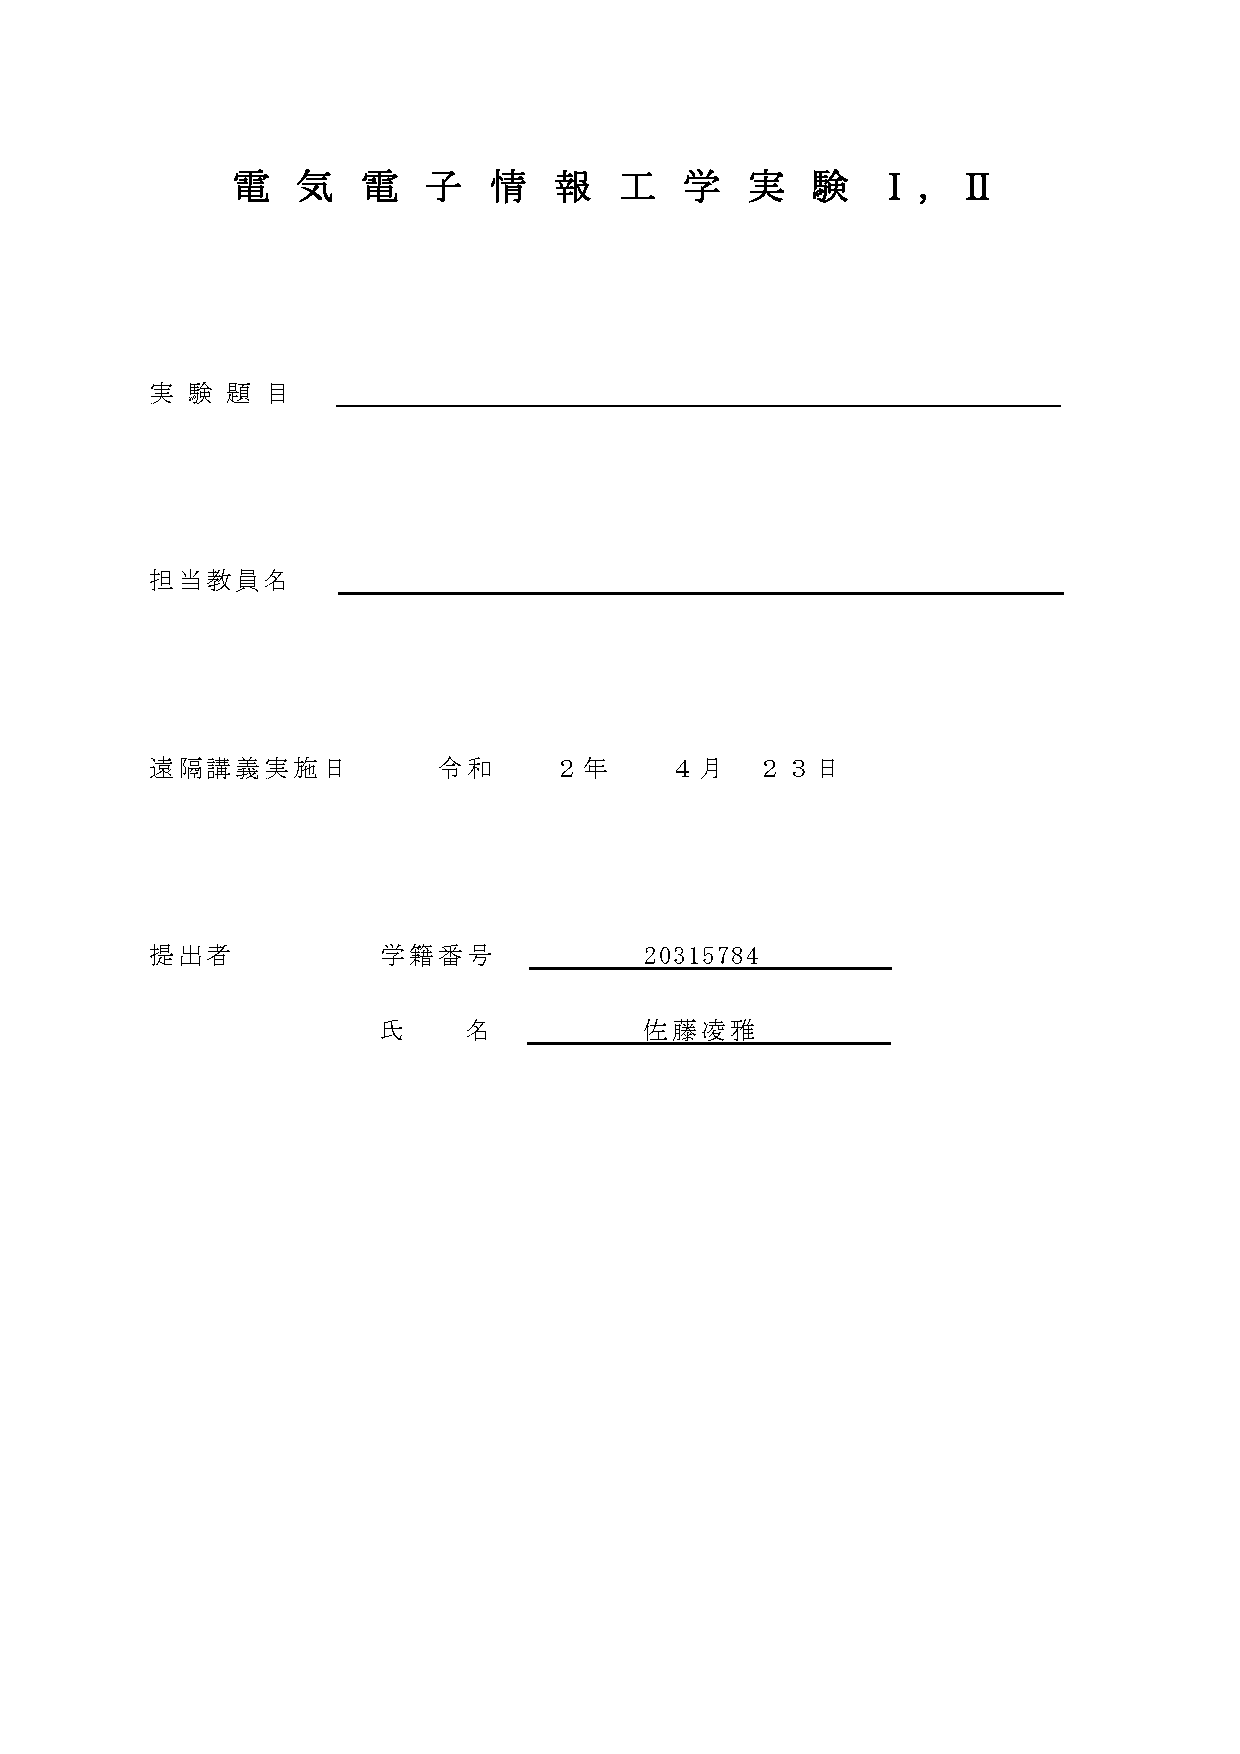
\includepdf[pages=-]{./setting/cover.pdf}
\maketitle

\fontsize{11.041pt}{16.562pt}\selectfont

\section{概要 Abstract}
 実験の目的、手段、結果、結論を簡潔にまとめ示すこと。(250字程度)

\section{目的 Purpose}
 テキストに書かれている目的等を参考に、各自どの点に注目して実験したのかを明確に示すこと。(300字程度)

\section{理論的背景 Theory}
 各自の実験目的に必要な理論的な背景を示すこと。必要ならば、参考文献リストより文献番号を引用すること。(レポート用紙1枚程度)

\section{実験方法 Experiment}
 実験手段、測定系の概要、測定装置の名称・型番等を書くこと。また、装置の精度・仕様等の情報もできる限り示すこと。(レポート用紙2枚程度)

\section{実験結果 Results}
 各自の実験目的に沿った結果を簡潔にまとめること。その他の試行錯誤的実験データは Appendix にまとめる。枚数は各教員の指示に従ってください。(レポート用紙の枚数は教員の指示に従う)

\section{考察 Discussion}
 各自の目的と照らし合わせ、測定結果の妥当性や数値計算結果との整合性などについて考察する。実験結果とサブテキスト/参考書の図式とを比較し議論すること。課題が与えられているテーマに関してはそれについても考察すること。(レポート用紙2枚程度)

\section{工夫した点}
 君自身が実験を通じて(実験の方法、まとめ方などで)工夫した点をまとめる。(100字程度 )

\section{結論 Conclusion}
 実験結果の羅列ではなく、考察した結果をまとめること。(250字程度)

\section{参考文献 Reference}
 レポートで引用した参考文献のリストを付ける。

\appendix
\section{Appendix}
 周辺の関連調査事項、作成プログラムリスト、試行錯誤的実験データ

\end{document}
